\documentclass[a4paper,11pt]{article}

\usepackage[slovene]{babel}
\usepackage[T1]{fontenc}
\usepackage[utf8]{inputenc}
\usepackage{lmodern}

\usepackage{textcase,float}
\usepackage{amsmath}
\usepackage{amsfonts}
% \usepackage{amsthm}
\usepackage{fancyhdr}
\usepackage[italicdiff]{physics}
\usepackage{url}
\usepackage{graphicx}
\usepackage{bm}
\usepackage{physics}
\usepackage{icomma}
\usepackage{hyperref}
%\usepackage{palatino}
\DeclareMathOperator{\N}{N}
\usepackage[margin=1in]{geometry}

\graphicspath{ {./images/}}

\pagestyle{fancy}
\fancyhf{}
\rhead{\thepage}
\lhead{\textsc{\textsc{Seminarska naloga iz statistike}}}

% \setlength{\parskip}{1em}

\newcommand{\ols}[1]{\mskip.5\thinmuskip\overline{\mskip-.5\thinmuskip {#1} \mskip-.5\thinmuskip}\mskip.5\thinmuskip} % overline short
\newcommand{\olsi}[1]{\,\overline{\!{#1}}} % overline short italic

\newcommand{\sumin}{\sum_{i = 1}^n}
\newcommand{\sumiN}{\sum_{i = 1}^N}

\newcommand{\inv}{^{-1}}
\newcommand{\prob}{\mathbb{P}}

\newcommand{\R}{\mathbb{R}}
\newcommand{\Z}{\mathbb{Z}}

\AtBeginDocument{
    \renewcommand{\var}[1]{\operatorname{var}(#1)}
}
    
\DeclareMathOperator{\se}{se}
\DeclareMathOperator{\bin}{Bin}

%%%%%%%%%%%%%%%%%%%%%%%%%%%%%%%%%%%%%%%%%%%%%%%%%%%%%%%%%%%%%%%%

\begin{document}
    
\author{\Large{\textbf{Nik Globočnik}}}
\title{SEMINARSKA NALOGA IZ STATISTIKE}
\date{4.~februar 2023}

\maketitle
\thispagestyle{empty}

\par
Seminarska naloga iz statistike pri predmetu Statistika na Fakulteti za matematiko in fiziko v Ljubljani v študijskem letu 2021/22. Link do repozitorija:
\begin{center}
    \url{https://github.com/nekineki} 
\end{center}

%-------------------------------------------------------------%
\section*{1. naloga - Kibergrad}
%-------------------------------------------------------------%
\noindent\textbf{a)} Narisali sem histogram dohodkov družin v Kibergradu. Širino posameznega razreda smo določili s pomočjo Friedman-Diaconiosvega pravila. Širina razreda je po tem pravilo podana kot
\[
    \ell = \frac{2(q_{3/4}-q_{1/4})}{\sqrt[3]{n}},
\]
kjer je $n$ število enot. Širino razreda pa smo potem smiselno zaokrožil na $\ell = 2000$. Število razredov smo določil po formuli
\[
    \#\text{razredov} = \left\lceil \frac{\max (\text{dohodki})-\min (\text{dohodki})}{\ell}\right\rceil
\]
in dobili, da je le to enako 238.
\newline 

\begin{figure}[H]
    \centering
    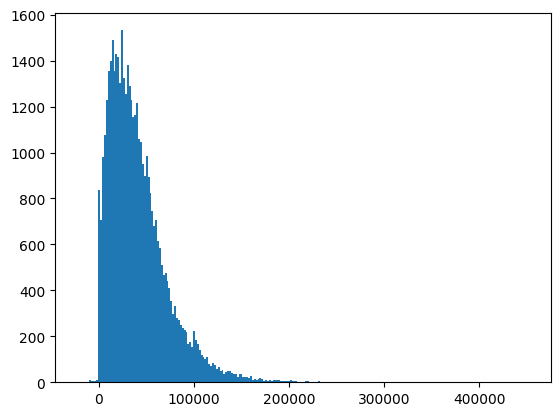
\includegraphics[scale = 0.5]{slike1/1_1.png}
    \caption{Histogram dohodkov}
\end{figure}


\noindent
\textbf{b)} Z vgrajenimi funkcijami smo izračunal povprečje dohodkov, ki je približno $\mu \approx 41336$, in standardni odklon, ki je približno $\sigma \approx 32038$. Zgornjemu histogramu smo dorisali graf normalne gostote $\N(\mu,~\sigma^2)$. Opazimo, da se graf normalne gostote ne prilega dobro histogramu, zato lahko sklepamo, da dohodki niso porazdeljeni normalno. Opazimo še, da je gospodinjstev s prihodki manjšimi od povprečja več, kot gospodinjstev z nadpovprečnimi dohodki.
\newline 

\begin{figure}[H]
    \centering
    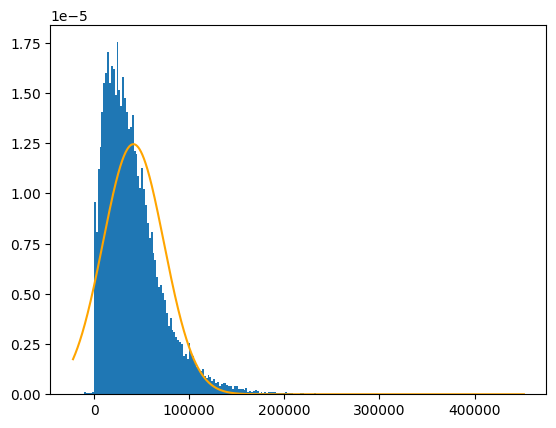
\includegraphics[scale = 0.5]{slike1/1_2.png}
    \caption{Histogram dohodkov z dorisano normalno gostoto}
\end{figure}


\noindent
\textbf{c)} Grafu kumulativne porazdelitvene funkcije porazdelitve dohodkov smo dorisali graf normalne kumulativne funkcije z že vgrajeno funkcijo \texttt{stat.NormalDist(mean, std).cdf()}.

\begin{figure}[H]
    \centering
    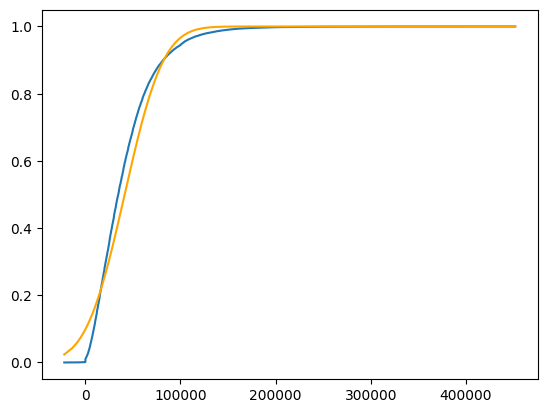
\includegraphics[scale = 0.5]{slike1/1_3.png}
    \caption{Primerjava kumulativne porazdelitvene funkcije porazdelitve prihodkov družin in normalne kumulativne funkcije}
\end{figure}

\noindent Vidimo, da se grafa pri visokih dohodkih dobro prilegata, kar lahko razberemo že iz Slike 2. Pri nižjih dohodkih pa opazimo odstopanje.
\newline


\noindent
\textbf{d)} Narisali smo primerjalni Q-Q grafikon. Če bi bili prihodki družin porazdeljeni normalno, bi se ročka prilegale simetrali lihih kvadrantov (dorisani z oranžno). Opazimo, da se podatki ne prilegajo, torej lahko spet sklepamo, da prihodki niso porazdeljeni normalno.
\newline

\begin{figure}[H]
    \centering
    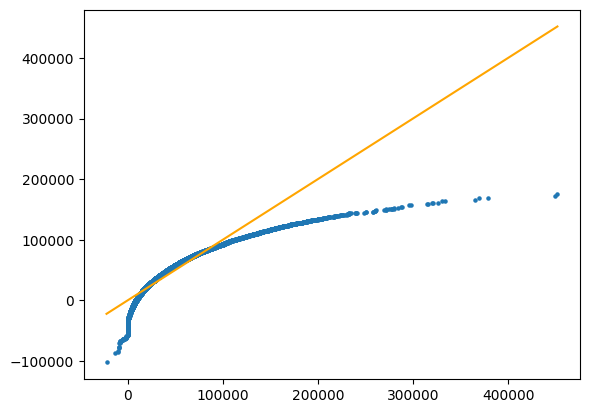
\includegraphics[scale = 0.5]{slike1/1_4.png}
    \caption{Primerjalni Q-Q grafikon}
\end{figure}

\noindent
\textbf{e)} Vzeli smo $1000$ slučajnih vzorcev velikosti $100$. Pri izračunu smo si pomagali z že vgrajeno funkcijo \texttt{sample()}. S pomočjo Friedman-Diaconiosvega pravila sem nato določili širine razredov in narisal histogram vzorčnih povprečij.
\newline

\begin{figure}[H]
    \centering
    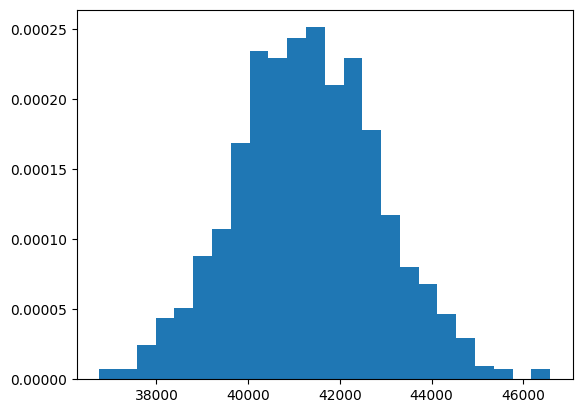
\includegraphics[scale = 0.5]{slike1/1_5.png}
    \caption{Histogram vzorčnih povprečij}
\end{figure}

\noindent
\textbf{f)} Da lahko histogramu vzorčnih povprečij dorišemo normalno gostoto izračunamo pričakovano vrednost, ki se ujema s povprečnim dohodkom, in standardno napako za enostavni slučajni vzorec velikosti $400$. Standardno napako za enostavni slučajni vzorec lahko izračunamo po formuli 
\[
    \operatorname{SE}^2 = \frac{N-n}{N-1}\cdot\frac{\sigma^2}{n},
\]
kjer je $N$ velikost celotne populacije, $n$ velikost slučajnega vzorca in $\sigma^2$ standardni odklon prihodkov celotne populacije. 


\begin{figure}[H]
    \centering
    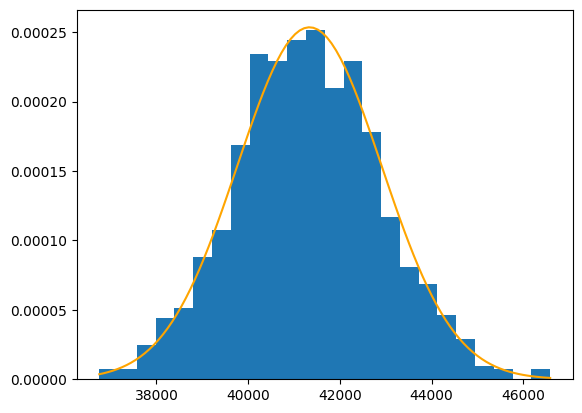
\includegraphics[scale = 0.5]{slike1/1_6.png}
    \caption{Histogram vzorčnih povprečij z dorisano normalno gostoto}
\end{figure}

\noindent Opazimo, da se graf te normalne porazdelitve dobro ujema s histogramom vzorčnih povprečij. 
\newline

\noindent
\textbf{g)} Podobno kot zgoraj narišemo kumulativno porazdelitveno funkcijo in Q-Q grafikon z avzorčna povprečja. Opazimo zelo dobro prileganje v obeh primerih, torej lahko sklepamo, da ima vzorčno povprečje skoraj normalno porazdelitev. Omenimo še, da pride pri vsakem ponovnem zagonu programa do drugačne izbire slučajnega vzorca in zato tudi do novih izračunov standardne napake. Ob slabi izbiri slučajnega vzorca lahko pride tudi do odstopanj od normalne porazdelitve.
\newline

\begin{figure}[H]
    \centering
    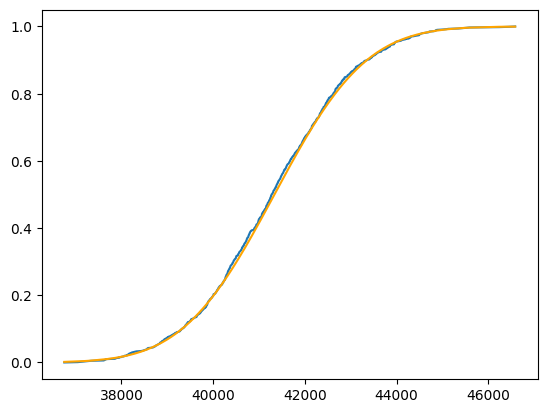
\includegraphics[scale = 0.45]{slike1/1_7.png}
    \caption{Primerjava kumulativne porazdelitvene funkcije za vzorčna povprečja prihodkov družin in normalne kumulativne funkcije}
\end{figure}

\begin{figure}[H]
    \centering
    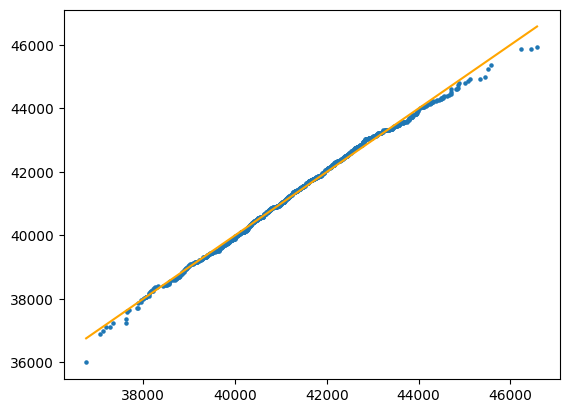
\includegraphics[scale = 0.45]{slike1/1_8.png}
    \caption{Q-Q grafikon vzorčnega povprečja prihodkov}
\end{figure}


%-------------------------------------------------------------%
\section*{2. naloga - Delnice}
%-------------------------------------------------------------%
\noindent
\textbf{a)} V podatkih smo dobili relativne mesečne donose delnic podjetij Halliburton in McDonalds med leti 1975 in 1999. Narisali smo histogram donosov, kjer smo širino razreda določili z modificiranim Freedman-Diaconisovim pravilom, ki pravi: 
\[
    \ell = \frac{2.6\cdot(q_{3/4}-q_{1/4})}{\sqrt[3]{n}}.
\]
Na histograma donosov smo potem dorisali še pripadajoči normalni porazdelitvi.

\begin{figure}[H]
    \centering
    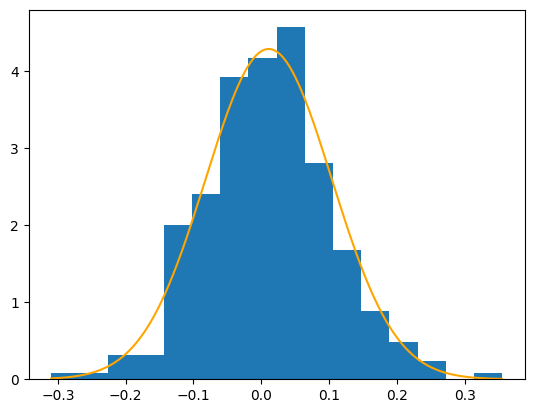
\includegraphics[scale = 0.45]{slike1/2_3.png}
    \caption{Halliburton: histogram donosov in dorisana normalna porazdelitev}
\end{figure}

\begin{figure}[H]
    \centering
    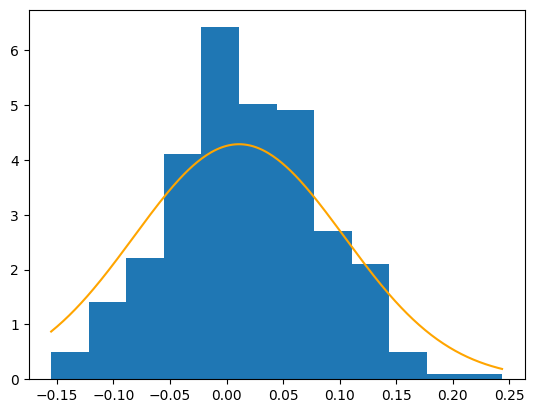
\includegraphics[scale = 0.45]{slike1/2_4.png}
    \caption{McDonalds: histogram donosov in dorisana normalna porazdelitev}
\end{figure}

\noindent Opazimo, da se donosi delnic podjetja Halliburton dobro prilegajo normalni porazdelitvi, delnice podjetja McDonalds pa manj. Bolj volatilna je delnica podjetja McDonalds, saj je njena pripadajoča normalna porazdelitev širša (večji standardni odklon). To pomeni, da ta delnica dozeže veliko večje razlike med pozitivnimi in negativnimi donosi, kot delnica podjetja Halliburton.
\newline

\noindent
\textbf{b)} Za vsako od delnic smo narisali še priemrjalni Q-Q grafikon.

\begin{figure}[H]
    \centering
    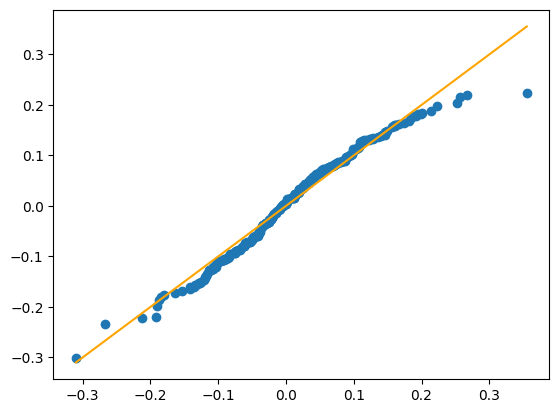
\includegraphics[scale = 0.45]{slike1/2_5.png}
    \caption{Q-Q grafikon; Halliburton}
\end{figure}

\begin{figure}[H]
    \centering
    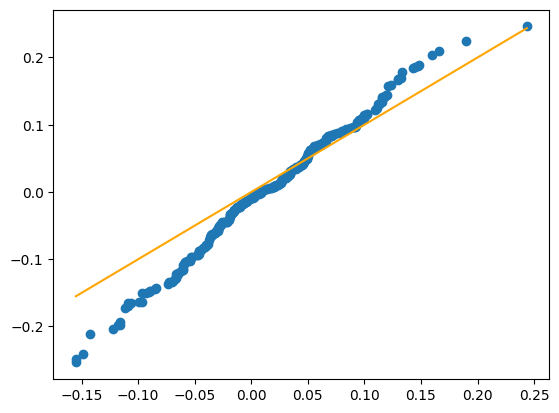
\includegraphics[scale = 0.45]{slike1/2_6.png}
    \caption{Q-Q grafikon; McDonalds}
\end{figure}

\noindent Tudi primerjalna Q-Q grafikona potrjujeta naše zgornje ugotovitve. Delnica podjetja McDonalds se razlikuje od normalne porazdelitve, delnica podjetja Halliburton pa se dobro ujema z normalno porazdelitvijo.



%-------------------------------------------------------------%
\section*{3. naloga - Zobje}
%-------------------------------------------------------------%

\noindent
\textbf{a)} 
Najprej preverjamo, če dodajanje vitamina C sploh vpliva na rast zob. Naj $X_i$ dolžino zoba morskega prašička pri dodajanju 0.5 vitamina C, $Y_j$ dolžino pri dodajanju 1.0 vitamina $C$ in $Z_k$ dolžino pri dodajanju 2-0 vitamina C; $i\in\{1,2,\dots,20\}$. Predpostavimo, da so $X_i$, $Y_i$ in $Z_i$ zaporedoma porazdeljene z $\N(\mu_X,\sigma^2)$, $\N(\mu_Y,\sigma^2)$ in $\N(\mu_Z,\sigma^2)$.

Najprej testiramo ničelno hipotezo 
\[ 
    H_0: \mu_Y = \mu_X 
\] 
proti enostranski alternativni hipotezi 
\[ 
    H_1: \mu_Y >\mu_X.
\]
Hipotezo preizkusimo s Studentovim $T$-testom na testni statistiki
\[
    T = \frac{\overline{Y}-\overline{X}}{s\sqrt{\frac{1}{n}+\frac{1}{m}}},
\]
kjer je 
\[
    s^2 = \frac{\sum_{i=1}^n (X_i-\overline{X})^2+\sum_{i=1}^m(Y_i-\overline{Y})}{n+m-2}.
\]
Izkaže se, da je $T\sim\operatorname{Student}(n+m-2).$ V našem primeru je $m=n=20$. Iz tabele za Studentovo porazdelitev pri stopnjah tveganja $0.05$ in $0.01$ odčitamo 
\[
    F^{-1}_{\operatorname{Student}(38)}(0.05) = 1.686 \; \text{ in } \; F^{-1}_{\operatorname{Student}(38)}(0.01) = 2.4286.
\]
Vrednost testne statistike pa izračunamo s pomočjo vgrajene funkcije \texttt{ttest.ind()}. Dobimo $T = 6.476647726589102$. Ker je $T > F^{-1}_{\operatorname{Student}(38)}(0.05)$ in $T > F^{-1}_{\operatorname{Student}(38)}(0.01)$ ničelno hipotezo zavrnemo pri stopnjah tveganja $0.05$ in $0.01$.

Enako naredimo še za preizkus ničelne hipoteze
\[ 
    H_0: \mu_Z = \mu_Y
\] 
proti enostranski alternativni hipotezi 
\[ 
    H_1: \mu_Z >\mu_Y.
\]
Tu dobimo $T = 4.90048431719355$. Spet lahko ničelno hipotezo zavrnemo tako za stopnjo tveganja $0.05$ kot za $0.01$. Od tud lahko sklepamo, da dodajanje vitamina $C$ res pozitivno vpliva na rast zob.
\newline 

\noindent
\textbf{b)} Označimo s $P_i$ dolžino zoba, če smo vitamin C dodajali s pomarančnim sokom in z $N_j$, če smo vitamin C dodajali neposredno. Testiramo ničelno hipotezo 
\[ 
    H_0: \mu_P = \mu_N
\] 
proti enostranski alternativni hipotezi 
\[ 
    H_1: \mu_P >\mu_N.
\]
Primer rešujemo analogno kot v \textbf{a)}. Izkaže se, da za našo testno statistiko velja $T\sim\operatorname{Student}(58)$. S programom izračunamo testno statistiko, ki znaša $T=1.91526826869527$.  Odčitamo še 
\[
    F^{-1}_{\operatorname{Student}(58)}(0.05) = 1.6716 \; \text{ in } \; F^{-1}_{\operatorname{Student}(58)}(0.01) = 2.3924.
\]
Ker je $T > F^{-1}_{\operatorname{Student}(58)}(0.05)$ lahko ničelno hipotezo pri stopnji tveganja $0.05$ zavržemo, torej je bolj učinkovit način dodajanja vitamina C s pomarančnim sokom. Za stopnjo tveganja $0.01$ pa je $T < F^{-1}_{\operatorname{Student}(58)}(0.01)$, zato ničelne hipoteze ne moremo zavreči.

Za stopnjo tveganja $0.05$ si poglejmo še, ali je napaka statistično značilna. Funkcija \texttt{ttest.ind()} nam vrne tudi $p$-vrednost, ki znaša $p=0.030196685612064244$. Ker je $p\leq0.05$, je razlika statistično značilna.




\begin{thebibliography}{99}

    \bibitem{Rice}
    J.~Rice, \emph{Mathematical statistics \& data analysis}, third edition, Duxbury, 2007.

    \bibitem{Welch}
    \emph{Student's $t$-test}, v: Wikipedia, The Free Encyclopedia, [ogled 3.~2.~2023], dostopno na \url{https://en.wikipedia.org/wiki/Student%27s_t-test}.
    
\end{thebibliography}

\end{document}